\chapter{强化学习的心理学} \label{chap:chap11}

在前面的章节中,我们仅基于计算考虑就提出了算法的想法。
在本章中,我们从另一个角度来看其中的一些算法:心理学的角度及其对动物如何学习的研究。
本章的目的是,首先,讨论强化学习的思想和算法与心理学家对动物学习的发现相对应的方式,其次,解释强化学习对动物学习研究的影响。
事实证明,强化学习提供的清晰形式主义将任务,回报和算法系统化,在理解实验数据,提出新的实验种类以及指出可能对操作和测量至关重要的因素方面非常有用。
长期优化回报的想法是强化学习的核心,这有助于我们理解动物学习和行为的其他令人困惑的特征。


强化学习与心理学理论之间的一些对应关系并不令人惊讶,因为强化学习的发展受到了心理学学习理论的启发。
然而,正如本书所述,强化学习从人工智能研究人员或工程师的角度探索理想化的情况,目的是用有效的算法解决计算问题,而不是复制或详细解释动物如何学习。
因此,我们描述的一些通信将各自领域中独立产生的想法联系起来。
我们认为这些接触点特别有意义,因为它们揭示了对学习很重要的计算原理,无论是通过人工还是通过自然系统学习。


在大多数情况下,我们描述了强化学习和学习理论之间的对应关系,这些理论是为了解释大鼠,鸽子和兔子等动物如何在受控实验室实验中学习而开发的。
在整个20世纪进行了数千次这样的实验,其中许多至今仍在进行中。
虽然有时被认为与心理学中更广泛的问题无关,但这些实验探索了动物学习的微妙特性,通常是由精确的理论问题驱动的。
随着心理学将重点转移到行为的更多认知方面,即思维和推理等心理过程,动物学习实验在心理学中的作用比以前少了。
但是,这项实验导致了学习原则的发现,这些原则在整个动物界都是基本的和广泛的,这些原则在设计人工学习系统时不应该被忽视。
此外,正如我们将看到的那样,认知处理的某些方面自然地与强化学习提供的计算视角相关联。


本章的最后一节包括与我们讨论的联系以及我们忽视的联系相关的参考文献。
我们希望本章鼓励读者更深入地探讨所有这些联系。
最后一节还讨论了强化学习中使用的术语与心理学术语的关系。
强化学习中使用的许多术语和短语都是从动物学习理论中借用的,但是这些术语和短语的计算/工程意义并不总是与其在心理学中的意义一致。


\section{预测和控制}


我们在本书中描述的算法分为两大类:预测算法和控制算法。
这些类别自然出现在强化学习问题的解决方法中。
在许多方面,这些类别分别对应于心理学家广泛研究的学习类别:经典或巴甫洛夫式条件作用和工具性或操作性条件作用。
由于心理学对强化学习的影响,这些对应关系并不完全是偶然的,但它们仍然引人注目,因为它们将来自不同目标的想法联系起来。


本书中介绍的预测算法估计的数量取决于代理环境的特征在未来的发展情况。
我们特别关注于估计代理在与环境交互时未来可能获得的回报量。
在这个角色中,预测算法是策略评估算法,它是改进策略算法的组成部分。
但预测算法不仅限于预测未来的回报;他们可以预测环境的任何特征(例如,参见Modayil,White和Sutton,2014)。
预测算法和经典条件反射之间的对应关系取决于它们预测即将到来的刺激的共同特性,无论这些刺激是否有益(或惩罚)。


仪器或操作条件实验的情况是不同的。
在这里,实验装置的设置是为了根据动物的行为给予动物喜欢的东西(奖励)或不喜欢的东西(惩罚)。
动物学会增加产生奖励行为的倾向,减少产生惩罚行为的倾向。
据说强化刺激取决于动物的行为,而在经典条件反射中则不然(尽管在经典条件反射实验中很难消除所有行为偶然性)。
仪器调节实验就像我们在第一章中简要讨论的那些启发桑代克效应定律的实验。
控制是这种学习形式的核心,它对应于强化学习的策略改进算法的操作。


在预测方面思考经典条件反射,在控制方面思考工具条件反射,是将我们的强化学习的计算观点与动物学习联系起来的起点,但实际上,情况比这更复杂。
经典条件作用比预测更多;它还涉及行动,控制模式也是如此,有时被称为巴甫洛夫控制。
此外,经典和工具性条件反射以有趣的方式相互作用,这两种学习都可能在大多数实验情况下进行。
尽管存在这些复杂性,但将经典/工具区别与预测/控制区别相结合是将强化学习与动物学习联系起来的方便的rst近似。


在心理学中,强化一词用于描述经典条件反射和工具条件反射的学习。
最初只指强化一种行为模式,也经常用于弱化一种行为模式。
被认为是行为改变原因的刺激被称为增强剂,它是否取决于动物以前的行为。
在本章的末尾,我们将更详细地讨论这个术语,以及它与机器学习中使用的术语的关系。


\section{经典条件反射}

在研究消化系统的活动时,著名的俄罗斯生理学家伊万·巴甫洛夫(IvanPavlov)发现,动物对某些触发刺激的先天反应可能会被与先天触发因素无关的其他刺激触发。
他的实验对象是经过小手术的狗,以准确测量其唾液re-ex的强度。
在他描述的一个案例中,这只狗在大多数情况下都不会流涎,但在喂食后约5秒钟,它会在接下来的几秒钟内产生约6滴唾液。
在几次重复呈现另一种刺激后,一种与食物无关的刺激,在这种情况下是节拍器的声音,在引入食物之前不久,狗对节拍器的声音做出了唾液分泌的反应,就像它对食物的反应一样。
“因此,唾液腺的活动被声音的冲动所激发,这是一种与食物完全不同的刺激”(巴甫洛夫,1927,第22页)。
巴甫洛夫总结了这一发现的重要性,写道:


很明显,在自然条件下,正常动物不仅必须对自身带来直接好处或伤害的刺激作出反应,而且还必须对其他物理或化学机构(声波,光波等)作出反应,这些物理或化学机构本身只发出这些刺激的接近信号;
虽然猎物的视觉和声音本身对较小的动物有害,但它的牙齿和爪子有害。(巴甫洛夫,1927年,第14页)


以这种方式将新刺激与先天性反应联系起来,现在被称为经典或巴甫洛夫条件反射。
巴甫洛夫(或者更确切地说,他的翻译人员)将先天性反应(例如,上述演示中的流涎)称为“无条件反应”(URs),其自然触发刺激(例如食物)“无条件刺激”(USs),以及由预测刺激触发的新反应(例如,这里还有流涎)“条件反应”(CRs)。
最初是中性的刺激,意味着它通常不会引起强烈的反应(例如节拍器声音),当动物知道它预测美国并因此产生CR以响应CS时,它就会成为“条件刺激”(CS)。
这些术语仍然用于描述经典的条件反射实验(尽管更好的翻译应该是“有条件的”和“无条件的”,而不是有条件的和无条件的)。
美国被称为强化者,因为它强化了对CS产生CR的反应。


右侧显示了两种常见类型的经典调节实验中刺激的排列。
在延迟调节中,CS延伸到整个刺激间隔或ISI,这是CS发作和美国发作之间的时间间隔(当美国以此处显示的常见版本结束时,CS结束)。
在跟踪条件反射中,US在CS结束后开始,CS o集合和US开始之间的时间间隔称为跟踪间隔。


\begin{figure}[!htb]
	\centering
	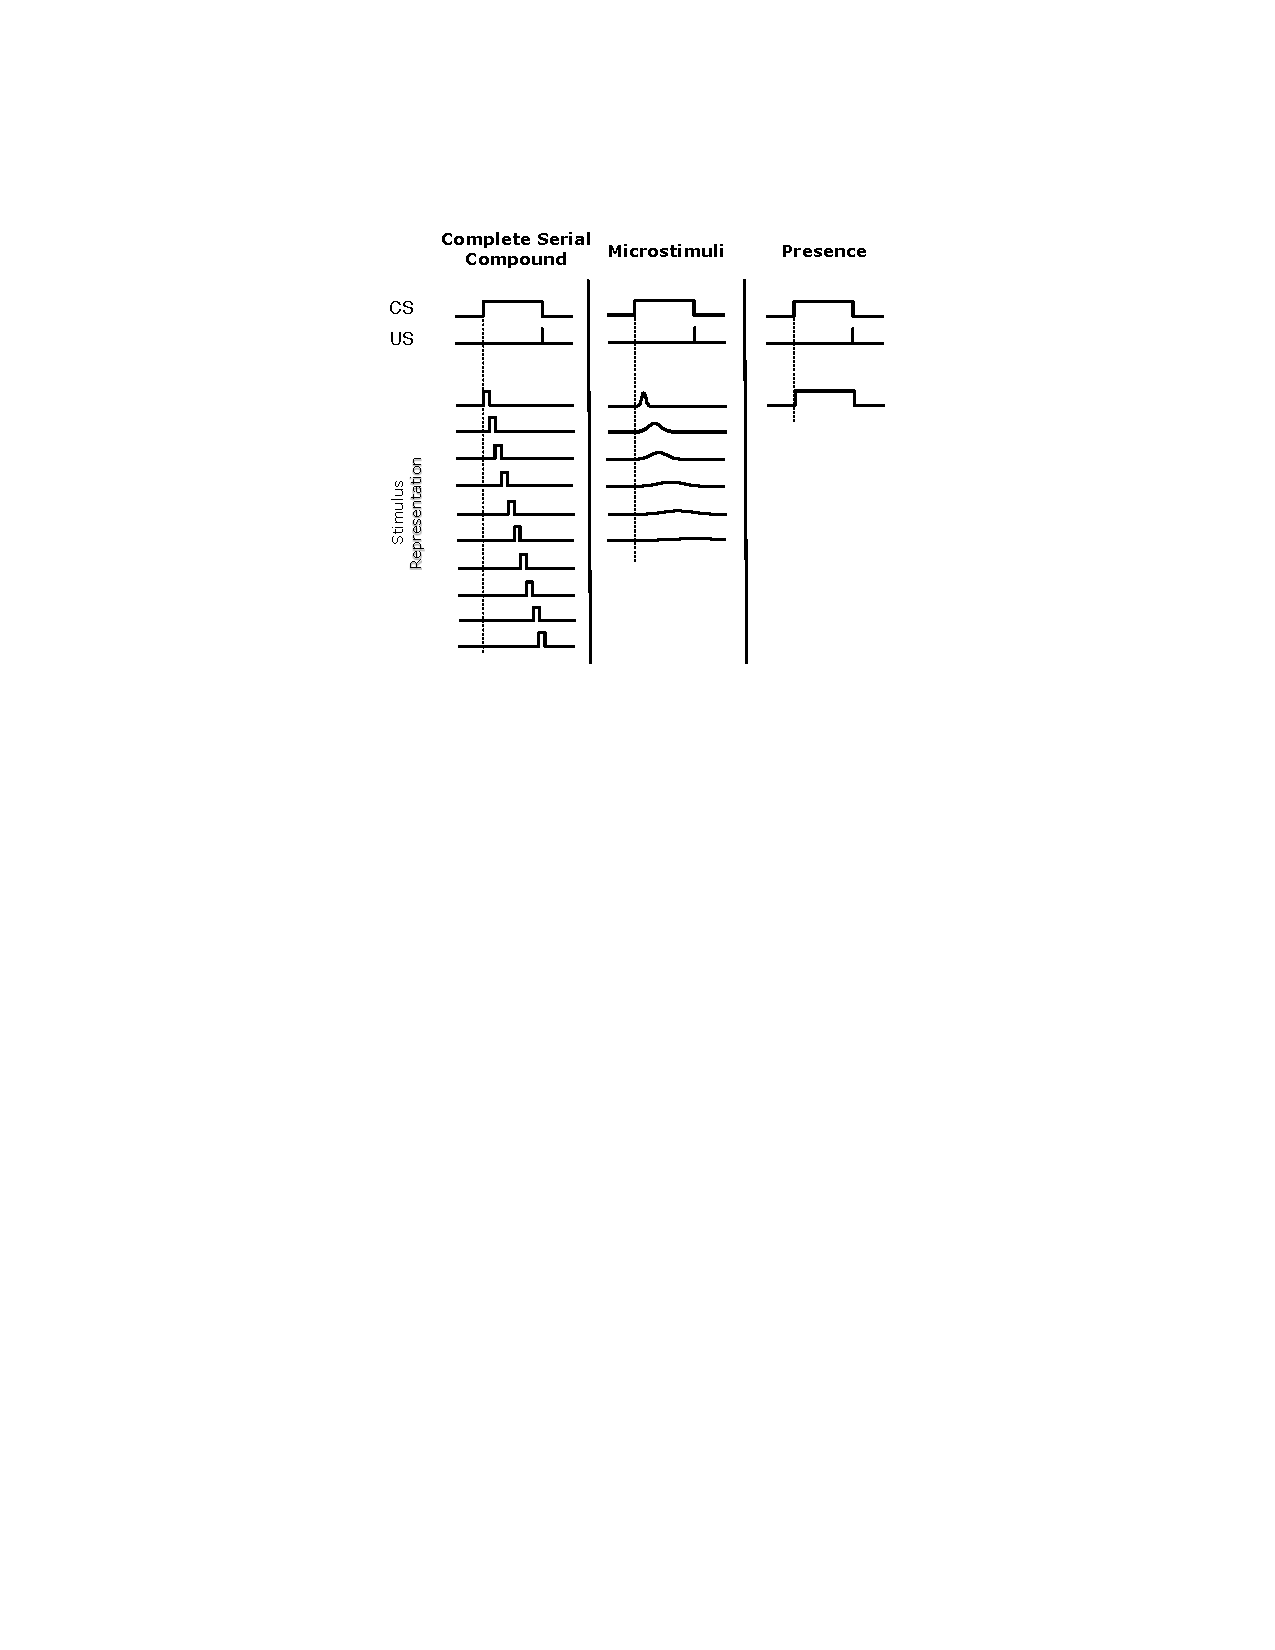
\includegraphics[width=0.5\linewidth]{chap11/fig_11_1}
	\caption{  \label{fig:11_1}}
\end{figure}


巴甫洛夫的狗对节拍器的声音流涎只是经典条件反射的一个例子,已经在许多动物的许多反应系统中进行了深入研究。
URs通常在某种程度上是准备性的,比如巴甫洛夫的狗流涎,或者在某种程度上是保护性的,比如对刺激眼睛的东西眨眼,或者看到捕食者时冻结。
在一系列试验中经历CS-US预测关系会使动物了解到CS预测美国,因此动物可以通过CR对CS做出反应,为动物做好准备或保护其免受预测的美国的影响。
一些CR类似于UR,但开始得更早,并且以增加其有效性的方式开始。
例如,在一项深入研究的实验中,音调CS可靠地预测了兔子眼睛的空气pu(美国),触发了UR,该UR由称为切口膜的保护性内眼睑闭合组成。
在一次或多次试验后,音调开始触发由膜闭合组成的CR,该膜闭合在空气pu之前开始并最终定时,以便在空气pu可能发生时发生峰值闭合。
这种CR是在预期空气pu和适当时间的情况下启动的,比简单地启动关闭作为对刺激我们的反应更好。通过学习刺激之间的预测关系来预测重要事件的能力是如此有益,它广泛存在于动物界。





\subsection{阻塞和高阶条件反射}

在实验中已经观察到经典条件反射的许多有趣性质。
除了CRs的预期性质之外,在经典调节模型的发展中,两个广泛观察到的特性得到了显着体现:阻塞和高阶调节。
当一个潜在的CS与之前用于调节动物产生CR的另一个CS一起出现时,当动物无法学习CR时,就会发生阻塞。
例如,在涉及兔子切口膜调节的阻断实验的第一阶段,兔子首先用音调CS和空气pu US调节,以产生在预期空气pu的情况下关闭其切口膜的CR。
实验的第二阶段包括额外的试验,其中第二个刺激(例如光)被添加到音调中以形成复合音调/光CS,然后是相同的空气pu US。
在实验的第三阶段,仅第二个刺激(即光)被呈现给兔子,以查看兔子是否已经学会了用CR对其作出反应。
结果表明,兔子对光的反应产生了很少或没有CR:对光的学习已经被先前对音调的学习所阻止。
2这样的阻止结果挑战了这样的观点,即调节只依赖于简单的时间连续性,即必要和足够的条件条件反射是美国经常在时间上紧跟CS。
在下一节中,我们将描述Rescorla{Wagner模型(Rescorla和Wagner,1972),该模型为阻塞提供了全面的解释。
	


当先前条件化的CS充当US来调节另一个最初中性的刺激时,就会发生高阶条件化。
如上所述,巴甫洛夫描述了一个实验,在这个实验中,他的助手首先调节一只狗,让它随着节拍器的声音流涎,节拍器可以预测食物的味道。
在这个调节阶段之后,进行了许多试验,其中将狗最初独立的黑色方块放置在狗的视线中,然后是节拍器的声音,而不是食物。
在仅仅十次试验中,这只狗只在看到黑色方块时才开始流涎,尽管事实上,看到它之后从来没有食物。
节拍器的声音本身就像一个US,将流涎的CR调节为黑色方块CS。
这是二阶条件反射。如果黑色方块被用作美国来建立另一个中性CS的唾液CRs,那么它将是三阶条件反射,等等。高阶条件反射很难证明,特别是在二阶以上,部分原因是高阶增强剂由于在高阶条件反射试验中没有被原美国反复遵循而失去了增强价值。
但是在正确的条件下,例如将一阶试验与高阶试验混合或通过提供一般的激励刺激,可以证明二阶以上的高阶条件反射。
正如我们在下面所描述的,经典条件反射的TD模型使用了自举思想,这是我们的方法的核心,以扩展Rescorla{Wagner模型对阻塞的描述,以包括CRs的预期性质和高阶条件反射。
	
	
	




















